\section{Xây dựng mô hình dự đoán}

Sau khi hoàn tất bước tiền xử lý dữ liệu, tập dữ liệu được chia thành hai phần: tập huấn luyện (training set) và tập kiểm tra (test set) theo tỷ lệ 80:20. Việc phân chia này nhằm đảm bảo mô hình được đánh giá trên dữ liệu chưa từng thấy, từ đó phản ánh chính xác khả năng tổng quát hóa.

\begin{figure}[h!]
	\centering
	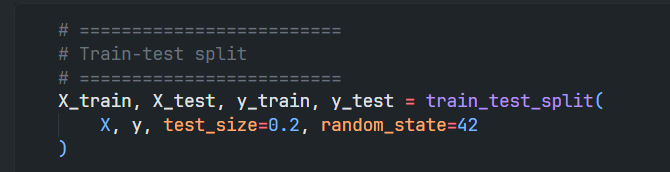
\includegraphics[width=1\linewidth]{chapters/Implement/ttsplit.png}
	\caption{Chia tập dữ liệu Train/Test}
\end{figure}

Mặc dù các đặc trưng trong tập dữ liệu đều ở dạng số, nhưng chúng có sự khác biệt lớn về thang đo. Điều này có thể ảnh hưởng tiêu cực đến hiệu quả của một số mô hình, đặc biệt là các mô hình tuyến tính.

Do đó, kỹ thuật chuẩn hóa dữ liệu \textbf{StandardScaler} được sử dụng để đưa các đặc trưng về cùng một phân phối với trung bình bằng 0 và độ lệch chuẩn bằng 1. Việc chuẩn hóa giúp cải thiện tốc độ hội tụ và độ ổn định trong quá trình huấn luyện.

\begin{figure}[H]
	\centering
	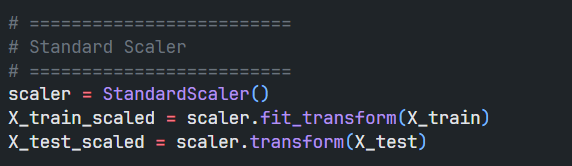
\includegraphics[width=1\linewidth]{chapters/Implement/scale.png}
	\caption{Chuẩn hóa dữ liệu với StandardScaler}
\end{figure}

Sau khi chuẩn bị dữ liệu, các mô hình được huấn luyện và đánh giá như sau:

\subsection{Hồi quy tuyến tính}

Mô hình hồi quy tuyến tính được huấn luyện trên dữ liệu đã được chuẩn hóa. Đây là mô hình cơ sở (baseline) nhằm thiết lập một mức tham chiếu cho hiệu suất của các mô hình phức tạp hơn.

\begin{figure}[H]
	\centering
	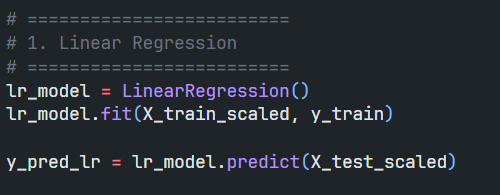
\includegraphics[width=0.5\textwidth]{chapters/Implement/linear.png}
	\caption{Mô hình hồi quy tuyến tính}
\end{figure}

\subsection{Random Forest}

Đối với mô hình Random Forest, nhóm sử dụng phương pháp \textbf{GridSearchCV} để tìm kiếm bộ siêu tham số tối ưu. Việc này giúp cải thiện hiệu suất mô hình một cách đáng kể.

Các siêu tham số được tinh chỉnh bao gồm:

\begin{itemize}
	\item \textbf{n\_estimators}: số lượng cây trong rừng
	\item \textbf{max\_depth}: độ sâu tối đa của cây
	\item \textbf{max\_features}: số đặc trưng được xét tại mỗi lần phân tách
	\item \textbf{min\_samples\_split}: số mẫu tối thiểu để chia node
	\item \textbf{min\_samples\_leaf}: số mẫu tối thiểu tại node lá
	\item \textbf{bootstrap}: sử dụng bootstrap sampling hay không
\end{itemize}

\begin{figure}[H]
	\centering
	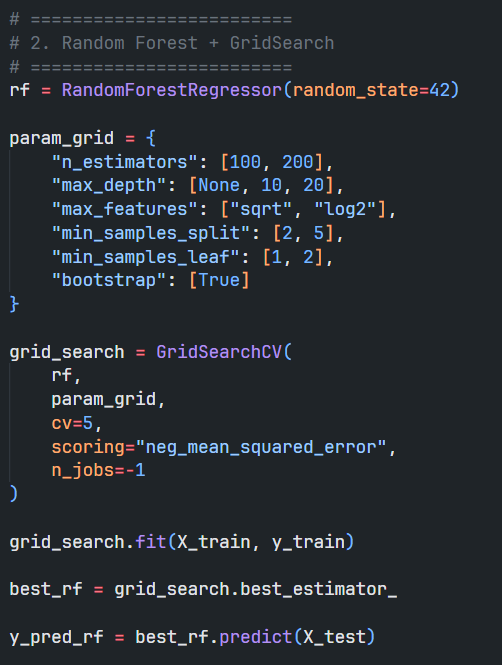
\includegraphics[width=0.8\linewidth]{chapters/Implement/GridCV.png}
	\caption{Tối ưu tham số với GridSearchCV}
\end{figure}

Sau quá trình tìm kiếm, mô hình thu được bộ tham số tối ưu giúp đạt hiệu suất tốt nhất trên tập validation.

\begin{figure}[H]
	\centering
	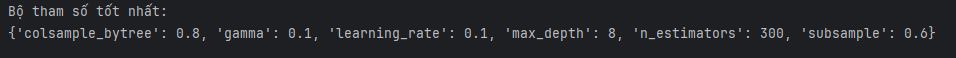
\includegraphics[width=0.8\linewidth]{chapters/Implement/BestParam.png}
	\caption{Bộ tham số tối ưu}
\end{figure}


\subsection{XGBoost}
Mô hình XGBoost được xây dựng và tối ưu hóa siêu tham số thông qua thuật toán tìm kiếm dạng lưới \texttt{GridSearchCV}. Quá trình này được kết hợp với phương pháp kiểm định chéo và sử dụng thang đo sai số toàn phương trung bình (Mean Squared Error - MSE) làm hàm mục tiêu đánh giá. 

Không gian tìm kiếm được thiết lập với các tham số cụ thể như sau:
\begin{itemize}
	\item \textbf{n\_estimators} (Tập giá trị thử nghiệm: \texttt{[100, 200, 300]}): Số lượng cây quyết định được xây dựng. Mỗi cây mới sẽ học cách bù đắp sai số cho các cây trước đó.
	
	\item \textbf{learning\_rate} (Tập giá trị thử nghiệm: \texttt{[0.01, 0.1]}): Điều chỉnh mức độ ảnh hưởng của mỗi cây mới lên mô hình cuối cùng. Giá trị nhỏ giúp mô hình hội tụ ổn định hơn và giảm thiểu rủi ro quá khớp (overfitting).
	
	\item \textbf{max\_depth} (Tập giá trị thử nghiệm: \texttt{[6, 8, 10]}): Chiều sâu tối đa của mỗi cây. Cây càng sâu càng nắm bắt được các quan hệ phi tuyến phức tạp, nhưng đồng thời làm tăng nguy cơ overfitting.
	
	\item \textbf{subsample} (Tập giá trị thử nghiệm: \texttt{[0.6, 0.8, 1.0]}): Tỷ lệ lấy mẫu ngẫu nhiên từ tập dữ liệu huấn luyện để xây dựng từng cây. Đặt giá trị nhỏ hơn 1 đóng vai trò như một kỹ thuật regularization.
	
	\item \textbf{colsample\_bytree} (Tập giá trị thử nghiệm: \texttt{[0.7, 0.8, 1.0]}): Tỷ lệ đặc trưng (features) được chọn ngẫu nhiên để huấn luyện tại mỗi cây, giúp các cây trong mô hình đa dạng hơn.
	
	\item \textbf{gamma} (Tập giá trị thử nghiệm: \texttt{[0.1, 0.3, 0.5]}): Ngưỡng giảm hàm mất mát tối thiểu yêu cầu để một node tiếp tục được phân nhánh. Đây là tham số quan trọng để kiểm soát độ phức tạp của cấu trúc cây.
\end{itemize}

% TODO: \usepackage{graphicx} required
\begin{figure}[H]
	\centering
	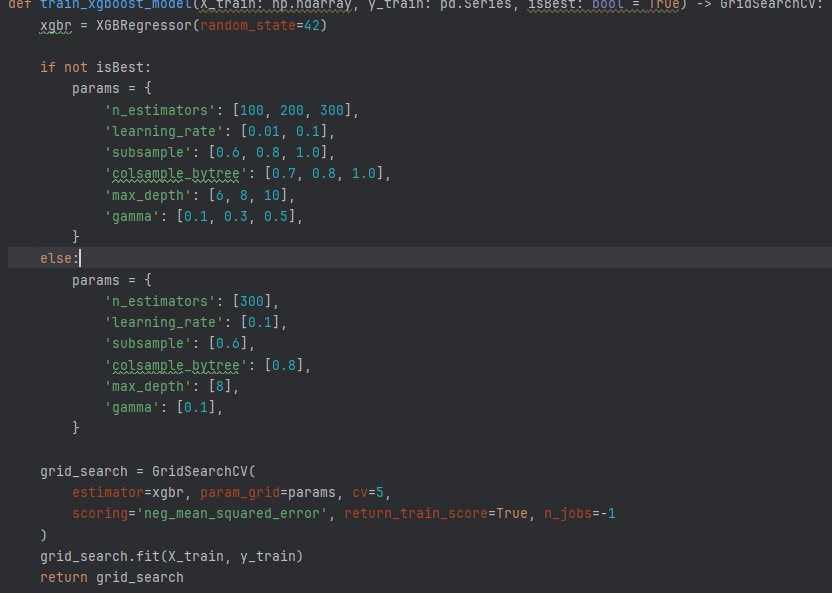
\includegraphics[width=0.8\linewidth]{chapters/Implement/CauhinhGrid}
	\caption{Cấu hình không gian tìm kiếm GridSearchCV cho XGBoost}
	\label{fig:cauhinhgrid}
\end{figure}

Sau khi rà soát toàn bộ các tổ hợp trong không gian siêu tham số, thuật toán đã hội tụ và xác định được bộ tham số tối ưu nhất, giúp mô hình đạt sai số thấp nhất trên tập kiểm định chéo. Kết quả bộ tham số tốt nhất được thể hiện như sau:

% TODO: \usepackage{graphicx} required
\begin{figure}[H]
	\centering
	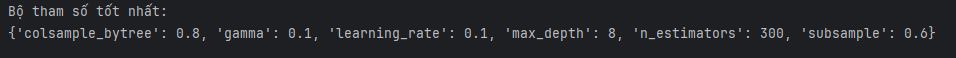
\includegraphics[width=0.8\linewidth]{chapters/Implement/BestParam}
	\caption{Bộ tham số tốt nhất cho mô hình}
	\label{fig:cauhinhgrid}
\end{figure}


\subsection{Mạng Nơ-ron nhiều lớp}
Ta tiến hành sử dụng phương pháp Nơ-ron nhiều lớp với cấu trúc như trong hình 5.8.
% TODO: \usepackage{graphicx} required
\begin{figure}[H]
	\centering
	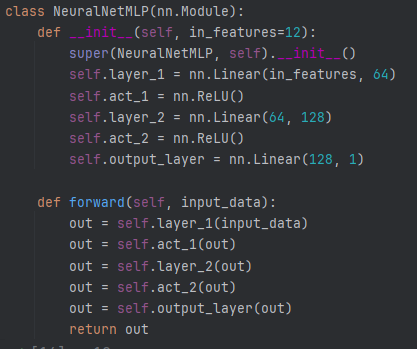
\includegraphics[width=0.6\linewidth]{chapters/Implement/MLP}
	\caption{Phương pháp mạng Nơ-ron nhiều lớp}
	\label{fig:mlp}
\end{figure}
Ta tiến hành huấn luyện mô hình với các tham số huấn luyện: 
\begin{itemize}
	\item Learning rate: 0.001
	\item Hàm mất mát: MSE
	\item Hàm tối ưu: Adam
	\item Số epoch: 35
\end{itemize}
Sau khi huấn luyện, ta tiến hành vẽ đồ thị mất mát. Thông qua đồ thị cho thấy cả Train Loss và Validation Loss đều giảm dần theo số epoch, với Train Loss giảm nhanh hơn trong 10 epoch đầu, sau đó cả hai đường ổn định từ epoch 20. Validation Loss luôn cao hơn Train Loss nhưng khoảng cách không lớn, chứng tỏ mô hình không bị overfitting nghiêm trọng. Đến khoảng 30-35 epoch, cả hai đường gần như không giảm thêm, đạt điểm hội tụ.
% TODO: \usepackage{graphicx} required
\begin{figure}[H]
	\centering
	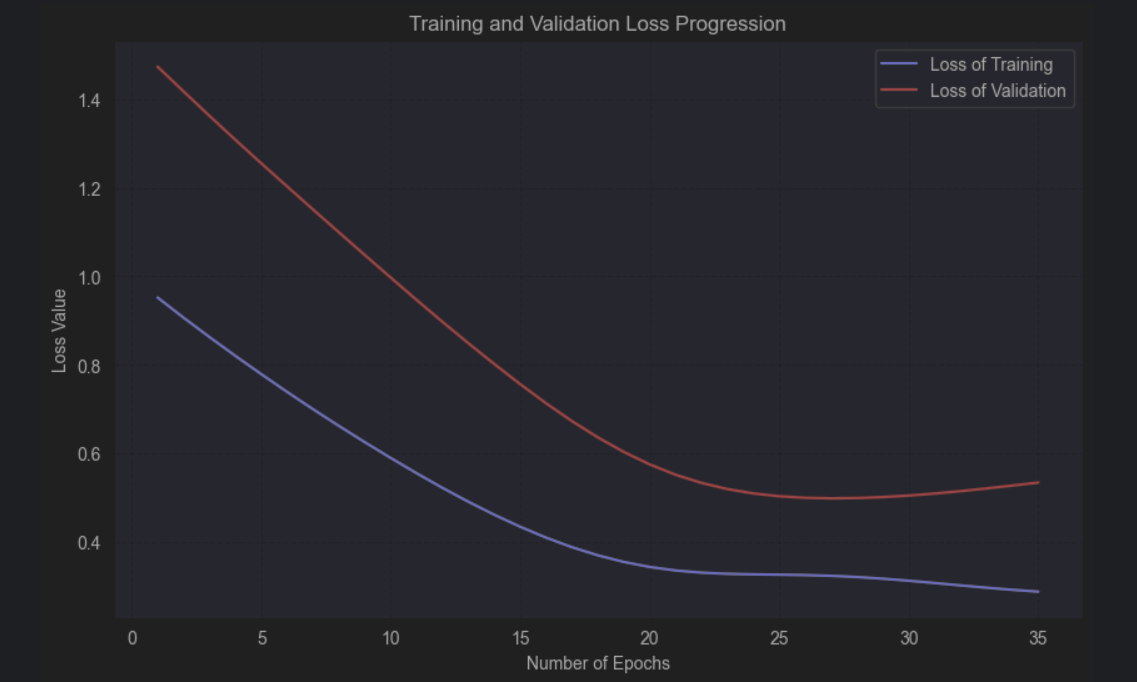
\includegraphics[width=0.8\linewidth]{chapters/Implement/Loss}
	\caption{Đồ thị mất mát}
	\label{fig:loss}
\end{figure}
